\documentclass[11pt,a4paper]{article}
\usepackage[utf8]{inputenc}
\usepackage{amsmath}
\usepackage{amsfonts}
\usepackage{amssymb}
\usepackage{graphicx}
\usepackage{fullpage}
\author{Axel Struys - Alexis Buckens}
\title{Projet - Analyse des données}
\usepackage{listings}
\usepackage{adjustbox}
\usepackage{url}
\usepackage{placeins}
\usepackage{subfigure}
\lstloadlanguages{R}
\begin{document}
\maketitle

\section{Introduction}

Nous avons choisi une base de données en provenance de l'UCI Machine Learning Repository. Celle-ci est composée d'échantillons de vins rouges portuguais, ayant une appelation d'origine contrôlée ``Vinho Verde''. Ce vin provient du nord ouest du Portugal, réparti en 9 sous-régions ayant des sols et des climats différents. \footnote{\url{http://www.vinhoverde.pt/}} Cet éclatement de la production de ce vin à pour conséquence une grande variabilité des propriétés des différents échantillons. Dans ce dataset, chaque observation représente les différentes analyses physico-chimiques d'un échantillon de vin distinct, associées à une évaluation subjective, par un \oe nologue, de la qualité de ce vin.

\subsection{Description des variables}
Afin de mieux comprendre les analyses ultérieures, nous allons brièvement décrire les variables et ce qu'elles représentent. \footnote{Les informations de cette section sont tirées de  \url{http://www.calwineries.com/learn/wine-chemistry}}

\begin{description}
	\item[Fixed acidity (g/L)] Cette variable représente la concentration en acide tartarique présente dans le vin. C'est l'acide primaire présent dans les grappes de raisins, et son rôle est très important dans le goût du vin. De plus, il permet de contrôler la prolifération bactérienne en agissant comme conservateur.
	\item[Volatile acidity (g/L)] C'est une mesure de l'acide acétique présente dans le vin. Cette acide est produite par l'activité métabolique des bactéries et levures. Notamment, elle provient de la métabolisation de l'éthanol par les bactéries acétiques. La concentration doit être idéalement de 0,3g/L; Une plus haute concentration peut altérer l'expérience gustative en donnant un goût sûr au vin. 
	\item[Citric acid (g/L)] C'est un composant intermédiaire du cycle de l'acide citrique, permettant aux bactéries et aux levures de produire de l'énergie. Normalement, presque toute l'acide citrique est consommée durant la fermentation du vin, mais les vignerons peuvent en ajouter afin de donner un goût frais au vin. 
	\item[Sulfur dioxide (mg/L)] Le dioxide de soufre est un sous-produit de la fermentation, mais il est aussi utilisé comme additif par les vignerons. Il régule la croissances des bactéries et levures. Mais son intérêt majeur réside dans ses propriétés antioxidantes. En effet, le vieillissement du vin produit de l'acetaldehyde, molécule qui à l'odeur d'une pomme brunie. Le dioxide de souffre va se lier avec cette molécule, la rendant inodore. Le dioxide de souffre permet donc de préserver le goût fruité du vin. Néanmoins, trop de dioxide de soufre donne une odeur soufrée au vin, irritant les parois nasales. Il est présent à la fois sous forme dissoute et sous forme gazeuse (free sulfur dioxide).
	\item[Density (g/mL)] C'est la masse du vin par unité de volume. L'éthanol étant peu dense (0.789 g/mL), plus un vin est alcoolisé, moins il est dense. 
	\item[Résidual sugar (g/L)] Ce sont les sucres restant après la fermentation du sucre en alcool par les bactéries et levures. Ceci permet de distinguer un vin sec (>4g/L) d'un vin moelleux (entre 12 g/L et 45 g/L). Le sucre à une grande importance dans les caractéristiques sensorielles du vin, permettant de balancer son amertume et donnant un goût fruité agréable.
	\item[pH] Mesurant l'acidité, le pH ne corrèle pas totalement avec les autres variables représentant l'acides, car il est une mesure totale de l'acidité, incluant d'autres acides mineurs non représentés dans ce dataset.
	\item[Chlorides (g/L)] C'est la concentration en ions chlorures dans le vin. Ils proviennent de la dissolution du chlorure de sodium (sel). Ils contribuent au goût salé du vin, mais trop de sel peut influencer négativement le goût.
	\item[Sulphate (sulphate de potassium) (g/L)] C'est un engrais qui permet de compenser le manque en potassium du sol, favorisant la croissance des vignes. En outre, le sulphate est nécessaire pour la synthèse des protéines de la plante, et à un rôle bénéfique dans la formation de sucres et des composés organoleptiques (qui ont un rôle dans la perception du goût). Il a un effet sur les niveaux de sucres et donc d'alcool.
	\item[Alcohol (vol.\%)] \'Element essentiel du vin, l'éthanol est le produit attendu de la fermentation des levures. Avec le sucre, l'alcool est responsable du goût sucré du vin, et est évidemment un facteur important dans la dégustation de ce vin. Néanmoins, un volume trop important d'alcool peut dégrader l'expérience sensorielle.
	\item[Quality] C'est l'évaluation subjective, par des experts, de la qualité de l'échantillon de vin. C'est une variable discrète, dont le minimum est 0, et le maximum est 10. Dans l'échantillon sélectionné, celle-ci s'étend entre 3 et 8.
\end{description}

\subsection{Intérêt des méthodes factorielles dans ce projet}

La description des variables nous montrent que beaucoup peuvent influencer la qualité d'un vin, mais aussi, il apparaît qu'elles peuvent s'influencer entre elles. Aussi, il peut sembler plus adéquat de choisir un modèle d'entrée-sortie tel qu'une régression linéaire sur la qualité. Néanmoins, nous pensons que l'utilisation de méthodes factorielles peut présenter plusieurs avantages dans ce dataset.

Premièrement, les méthodes factorielles sont surtout descriptives. Ainsi, elles peuvent être considérées comme une des premières étapes dans la compréhension des données à analyser, nous permettant une analyse exploratoire des données.
Deuxièmement, nous nous trouvons dans une situation où il y a beaucoup de variables, et il est possible que nous nous trouvons dans une situation où beaucoup de ces variables covarient ensemble. Ceci pose des problèmes évidents de multicolinéarités dans l'hypothèse où nous souhaitions utiliser un modèle linéaire ultérieurement.
Enfin, ces méthodes nous permettent de représenter ces variables sur un plan de plus petite dimension, permettant une compréhension plus simple et intuitive des données.



\section{Méthodologie}

L'échantillon original était composé de 1689 observations. Chaque observation représente un échantillon d'un vin différent; Elles sont donc indépendantes. Une lacune dans cette base de donnée est que les auteurs ont choisi, pour des raisons de confidentialités, d'occulter l'origine et la marque de ces échantillons. Afin de simplifier les analyses, nous avons décidé en accord avec l'assistant de réduire la taille du dataset. En procédant à un échantillonnage (voir code en annexe), nous avons sélectionné 200 observations.

Nous allons séparer notre analyse en 4 parties. Dans la première partie, nous allons présenter quelques statistiques descriptives. Ensuite, nous procéderons à une analyse en composantes principales sur toutes les variables, sauf Quality. Ensuite, nous réaliserons une analyse des correspondances multiples en discrétisant certaines variable, et en incluant la variable quality. Enfin, nous procéderons à une analyse de clustering, afin de voir si les variables permettent de séparer naturellement les échantillons en fonction de leur qualité  

Avant de procéder à l'analyse proprement dite, il convient de rapidement préparer nos données. Tout d'abord, comme nous ne disposons que de variables continues, il est nécessaire de transformer certaines d'entre elles en variables discrètes afin de pouvoir ultérieurement procéder à la l'analyse en correspondance multiples. De plus, cela nous permettra d'analyser de manière plus adéquate les variables dont la relation n'est pas linéaire (voir scatterplot matrix figure \ref{fig:scatterplot}). Cette transformation peut être faite en séparant les valeurs des 5 premières variables du dataset, à savoir fixed.acidity, volatile.acidity, citric.acid, residual.sugar and chlorides en 5 intervalles et en attribuant chaque intervalle a une catégorie. 


\section{Statistiques descriptives}

\begin{table}[ht]
	\centering
	\begin{tabular}{lrrrrr}
		\hline
		& Mean & Std.dev & Median & Min & Max \\ 
		\hline
		Fixed acidity (g/L) & 8.23 & 1.67 & 7.80 & 5.00 & 13.40 \\ 
		Volatile acidity (g/L) & 0.53 & 0.17 & 0.54 & 0.16 & 1.00 \\ 
		Citric acid (g/L) & 0.27 & 0.19 & 0.26 & 0.00 & 0.68 \\ 
		Residual sugar (g/L) & 2.45 & 1.12 & 2.20 & 1.20 & 8.80 \\ 
		Chlorides (g/L) & 0.08 & 0.04 & 0.08 & 0.04 & 0.47 \\ 
		Free Sulfur Dioxide (mg/L) & 14.69 & 8.92 & 13.00 & 3.00 & 45.00 \\ 
		Total Sulfur Dioxide (mg/L) & 43.48 & 32.73 & 35.00 & 7.00 & 278.00 \\ 
		Density (g/mL) & 0.997 & 0.002 & 0.997 & 0.992 & 1.002\\ 
		pH & 3.31 & 0.14 & 3.33 & 2.94 & 3.72 \\ 
		Sulphates (g/L) & 0.64 & 0.13 & 0.62 & 0.37 & 1.31 \\ 
		Alcohol (vol. \%) & 10.49 & 1.06 & 10.20 & 9.00 & 14.00 \\ 
		Quality & 5.65 & 0.83 & 6.00 & 3.00 & 8.00 \\ 
		\hline
	\end{tabular}
	\caption{Statistiques descriptives (Moyenne, Ecart-type, mediane, minimum et maximum) des 12 variables}
	\label{table:statdesc}
\end{table}

La table \ref{table:statdesc} présente les statistiques descriptives des variables du dataset.
Dans l'annexe \ref{sec:normalite} se trouvent les boxplots, histogrammes, qq-plots, scatterplot matrix et tests de Shapiro-Wilk de la normalité des variables. Nous pouvons constater que seules les variables density et pH ont une distribution qui suit une loi normale. En outre, la relation entre certaines variables n'est pas linéaire. Ceci est à prendre en compte pour l'analyse en composante principale, car l'hypothèse sous-jascente de cette méthode suppose une relation linéaire entre les variables. Etant donné cette non-normalité, ainsi que la non-linéarité de la relation entre certaines variables, nous avons choisi d'utiliser la corrélation de Spearman afin de décrire les relations entre ces variables (voir table \ref{table:cor} de l'annexe \ref{sec:cor}). 

\section{Analyse en composantes principales}

Nous allons commencer par nous intéresser aux variables continues en effectuant une ACP (toutes les variables sauf Quality). De plus, nous avons inclus la variable "quality" comme variable supplémentaire. Cet ajout n'influence pas le calcul de l'ACP, mais nous permettra de mieux interpréter les sortes de l'ACP.
Deux premières questions peuvent être posées : combien de dimensions faut-il pour capturer l'essentiel de l'information, et comment les différentes variables sont-elles projetées sur les axes factoriels de ces dimensions.

Afin de répondre à la première question, trois règles peuvent-être considérées pour retenir les composantes principales.
\subsection{Composantes principales à retenir}
\begin{enumerate}
	\item Retenir toutes les composantes dans la valeur propre est supérieure à 1. Sur le tableau \ref{table:eigpca} situé en annexe \ref{sec:eigpca}, nous voyons que les 4 premières composantes principales ont une valeur propre supérieure à 1.
	\item Retenir les composantes dont le pourcentage de variance est supérieur à 100/nombre de variables, dans ce cas, 8.3\%. Le tableau \ref{table:eigpca} nous montre que les 4 premières composantes sont à retenir
	\item Retenir les composantes situées avant un décrochement (``coude'') sur le graphe des pourcentages de variances (scree plot). Sur la figure  \ref{fig:screepca}, nous pouvons voir un net effondrement du pourcentage de variance expliquée a partir de la composante 4. Selon cette règle, il faudrait retenir uniquement les 3 premières dimensions
\end{enumerate}
\begin{figure}
	\centering
	\includegraphics[scale=0.6]{"screeplotpca"}
	\caption{Pourcentage de variance expliquée par chaque dimensions, en ordre décroissant}
	\label{fig:screepca}
\end{figure}

Nous avons décidés de retenir les 4 premières composantes principales pour la suite de l'analyse.

\subsection{Représentation graphique des variables}
Dans l'annexe \ref{sec:eigpca} se trouvent les coordonnées factorielles des variables ainsi que leur contribution à la construction des axes factoriels.

\begin{figure}
\centering
\includegraphics[width=\textwidth]{"pca2"}
\caption{Représentation graphique de la projection des variables sur les 4 premiers axes factoriels}
\end{figure}

\paragraph{Premier axe}Cet axe capture la plus grande partie de l'information. On peut constater que fixed.acidity, citric.acid et pH sont les variables les mieux représentées; Elles sont fortement corrélées avec cette dimension. On peut considérer que cet axe capture de manière générale l'acidité. C'est donc l'information la plus importante qui décrit notre dataset. Ceci semble normal étant donné que 3 variables décrivent l'acidité. Volatile.acidity est beaucoup moins bien représentée sur cet axe. Les vignerons souhaitent contrôler au maximum la concentration en acide acétique dans leur vin, tout en ayant une certaine quantité d'acide tartarique et d'acide citrique pour donner un meilleur goût au vin. De plus, l'acide acétique est produite par les micro-organismes, tandis que l'acide tartarique et l'acide citrique proviennent du raisin. Ainsi, ces acides ont une origine différente, qui explique cette différence de représentation sur ce premier axe. Étonnamment, la densité est bien représentée sur cet axe. Nous n'avons pas d'explications quant à cette observation.

\paragraph{Deuxième axe}Total.sulfur.dioxide et free.sulfur.dioxide sont les mieux représentées. Le dioxide de souffre est présent à la fois à l'état gazeux et dissous dans le vin. Ainsi, il peut passer d'un état à l'autre en fonction des conditions de pressions et de température. Il est donc normal que ces deux variables soient proches sur le plan. Alcohol et residual.sugar sont moins bien représentés sur cet axe, ayant une corrélation moyenne avec cet axe. On peut voir que les vecteurs de ces deux variables pointent dans des directions opposées: ceci est logique en regard de la fermentation. En effet, les levures transforment le sucre en alcool. Ainsi, plus il y a d'alcool, et moins il reste de sucre résiduel dans le vin. De plus, le dioxide de souffre est opposé à l'alcool sur cet axe. Ceci est normal étant donné son utilisation comme régulation de l'activité métabolique des levure. Ainsi, plus il y a de dioxide de souffre, moins les levures pourrons métaboliser de l'éthanol. Ces relations sont bien représentés par ce deuxième axe. On peut considérer que cet axe capture l'information liée à l'activité métabolique des levures

\paragraph{Troisème axe}Les variables alcohol et volatile.acidity sont les mieux représentées sur cet axe, ayant une corrélation moyennement forte avec l'axe ($r=0.6$ et $r=-0.58$). Cet axe semble capturer l'information liée à l'activité métabolique des bactéries acétiques. En effet, ces dernières transforment l'éthanol en acide acétique. Plus il y a d'éthanol dans le vin, et moins ces bactéries auront eu l'occasion de transformer celui-ci en acide acétique. Remarquons que sulfure.dioxide est opposé à volatile.acidity. Comme pour le deuxième axe, ceci est explicable par l'effet de régulation de l'activité des bactéries de cet additif. Ceci est justement représenté par la direction opposé des vecteurs représentant ces variables.

\paragraph{Quatrième axe}La variable chloride est fortement corrélée avec cet axe. Elle semble relativement indépendante des autres variables, étant quasi orthogonale avec les autres axes. Ceci indiquerait que la concentration en chlorure de sodium aurait peu d'influence sur les activités métaboliques des bactéries et levures, en tout cas dans les proportions observées dans cet échantillon.

Remarquons aussi que la variable quality est faiblement représentée par les axes de l'ACP. Ceci est normal étant donnée que cette variable n'a pas été prise en compte dans l'analyse factorielle, mais est juste représentée de manière graphique. Nous voyons qu'elle semble légèrement associée à alcohol, sulphates, residual.sugar et les variables représentant l'acidité fixe et citrique. Nous aurons l'occasion d'analyser plus correctement la variable quality avec les autres variables dans la section suivante.

Ce dataset présente les échantillons de vins de manière anonyme. Il est donc impossible de tirer des conclusions intéressantes par rapport à la projection des individus sur les axes factoriels. Par soucis de complétude, nous avons inclus ces projections en annexe \ref{sec:eigpca} (Figure \ref{fig:pcaind}).

\section{MCA}

L'étape suivante consiste à effectuer une analyse en correspondance multiple. Pour cette analyse nous avond besoin de variables discrètes. La variables "quality" étant déjà une variable discrète, elle sera naturellement utilisée. Pour ce qui est des autres variables, nous les sélectionnerons sur basedu nombres de levels qu'elles prennent si ont les considérait comme factors, afin de prendre celles qui naturellement semblent les plus proches d'une variable discrètes et sur base de la non-linearité de leur relations. Les variables selectionnées seront alcool, citric acid, residual.sugar et free.sulfur, et ces variables seront transformées en variables discrètes avec 5 catégories.

La première question est de savoir combien de  dimensions conserver. Pour répondre à cette question, on peut de nouveau utiliser les varleurs propres et d'inéresser aux dimensions avec les valeurs propres les plus élevées. Si on trace un graphique reprenant les valeurs propres, de la plus élevée à la plus faible, on obtient le graphique suivant : 

\begin{center}
\includegraphics[scale=0.4]{"mca-eigen"}
\end{center}

On peut donc constater que la proportion de variance expliquée par les différentes dimensions décroît lentement. Puisqu'il nous faut choisir un nombre de dimensions restreint pour expliquer nos données, il nous faut choisir également un critère de décision. Un premier critère est celui du "coup de coude" : Il s'agit de choisir le nombre de dimension à partir duquel la valeur des valeurs propres décroit brusquement. Un "coup de coude" peut être trouvé a plusieurs endroits, entre autre aux alentours de la 4eme dimension (mais également après deux dimensions), mais en ne choisissant que 4 dimensions, on ne peut expliquer que 30\% de la variance. Un second critère consiste à choisir les dimensions pour lesquelles la valeur propres est supérieure à $\frac{1}{nbvar}$. Ce second critère nous pousse à choisir 10 dimensions, ce qui est fort élevé. On pourrait également choisir comme critère le \% de variance expliquée, en fixant par exemple le seuil à 60\%. Ce critère nous pousserait également à choisir 10 variables. On utilisera  donc au final les 4 premières dimensions.\bigskip

On peut également s'intéresser aux positions des individus, variables et categories dans les deux premières dimensions :

\begin{center}
\includegraphics[scale=0.6]{"biplot-mca"}
\end{center}

Sur ce graphique, on peut observer les catégories des variables (triangles rouges associés aux noms des variables), et les individus (ronds bleus). On peut ainsi voir quelles catégories/individus sont similaires. En l'occurence, le graphe est un peu difficile à comprendre du fait que la plupart des valeurs sont proches de l'origine, à l'exeption de deux outliers et des valeurs correspondant aux valeurs manquantes pour alcohol et residual.sugar qui s'en éloignent singulièrement. Néanmoins on peut déjà observer une certaine similarité entre les catégories "basses" de residual.sugar, citric.acid et alcohol, et on peut constater que alcohol "low" et alcohol "high" sont chacun à une des extremites de l'axe correspondant à la première dimension. La première dimension semble donc correspondre essentiellement au taux d'alcool dans le vin. On pourra vérifier cela ultérieurement en observant les contributions des différentes variables au premières dimensions. Finalement les vins de mauvaise qualité (4) se trouvent du coté gauche (alcohol low) tandis que les vins de bonne qualité (7) se trouvent du coté droit (alcohol high). \bigskip

On peut aussi ne s'intéresser qu'aux variables analysées et tracer un graphique des coordonnées des variables dans le plan formé par les deux premières dimensions :
%The squared correlations between variables and the dimensions are used as coordinates.
%Correlation entre variable discrete??
\begin{center}
\includegraphics[scale=0.6]{"plot-var-mca"}
\end{center}

Aucune des variables ne semble ici être particulièrement associée avec l'un ou l'autre axe. On peut aussi représenter graphiquement quelle catégorie est associée avec chacune des 5 premières dimensions grâce au graphique suivant  (agrandi en annexe) : 

%Correlation entre variable discrete??
\begin{center}
\includegraphics[scale=0.4]{"contrib"}
\end{center}

En conclusion, la MCA nous permet de réduire efficacement le nombre de dimensions, et les deux variables qui semblent être le plus étroitement associées sont le taux d'alcool et la qualité du vin.

\section{Clustering}

Il est également possible de regrouper les données en cluster sur base de la PCA. Différentes méthodes seront utilisées ici, toutes seront initialement appliquées aux résultats de la PCA. La première est la méthode ward, vue au cours, minimisant la perte d'information en décomposant l inertie du nuage de points. La seconde méthode sera le complete linkage et la troisième sera le complete linkage. Des graphiques représentant les cluster en couleurs, et les données dans le plan formé par les deux premières dimensions nous permettrons d'évaluer visuellement la pertinence de chacune des méthode. Le nombre de cluster  sélectionné sera celui choisi automatiquement par HCPC, et variera donc suivant la méthode utilisée. Les graphiques pour les trois méthodes (ward, complete linkage et single linkage respectivement) sont les suivants (agrandis en annexe):




\begin{center}

\includegraphics[width=.4\textwidth]{"single-pca"}


\includegraphics[width=.4\textwidth]{"complete-pca"}


\includegraphics[width=.4\textwidth]{"ward-pca"}


\end{center}


On peut voir que le single linkage n'est pas du tout satisfaisant : deux des clusters ne contiennent qu'un seul point tandis que le troisième cluster reprend l'ensemble des autres données. Le complete linkage est légèrement meilleur : les clusters 1 et 3 semblent avoir du sens, mais le cluster 4 ne comprend de nouveau qu'un seul point et le cluster 2 ne semble pas très homogène. La méthode de ward fournit de bien meilleurs résultats et nous obtenons ici des clusters qui semblent cohérents!


Une fois le clustering terminé, on peut passer à l'analyse discriminante et s'intéresser à comment classifier une nouvelles données dans ces catégories formées par clustering. Cette classification peut être faite en utilisant la fonction FDA fournie au TP, ou discrim.coa.




\section{Conclusion}

\newpage
\section{Annexes}
\appendix
\subsection{Matrice de corrélation}
\label{sec:cor}
\begin{table}[h]
	\centering
	\begin{adjustbox}{width=1\textwidth}
	\begin{tabular}{lrrrrrrrrrrrr}
		\hline
		& alcohol & chlorides & citric.acid & density & fixed.acidity & free.sulfur.dioxide & pH & quality & residual.sugar & sulphates & total.sulfur.dioxide & volatile.acidity \\ 
		\hline
		alcohol & 1.00 & -0.25 & 0.11 & -0.41 & -0.04 & -0.03 & 0.13 & 0.48 & 0.19 & 0.21 & -0.20 & -0.18 \\ 
		chlorides & -0.25 & 1.00 & 0.06 & 0.31 & 0.12 & 0.09 & -0.16 & -0.11 & 0.23 & -0.13 & 0.15 & 0.10 \\ 
		citric.acid & 0.11 & 0.06 & 1.00 & 0.43 & 0.63 & -0.17 & -0.57 & 0.27 & 0.16 & 0.36 & -0.00 & -0.62 \\ 
		density & -0.41 & 0.31 & 0.43 & 1.00 & 0.65 & -0.17 & -0.31 & -0.07 & 0.35 & 0.20 & 0.02 & -0.02 \\ 
		fixed.acidity & -0.04 & 0.12 & 0.63 & 0.65 & 1.00 & -0.23 & -0.70 & 0.09 & 0.20 & 0.22 & -0.06 & -0.20 \\ 
		free.sulfur.dioxide & -0.03 & 0.09 & -0.17 & -0.17 & -0.23 & 1.00 & 0.22 & 0.05 & 0.08 & 0.04 & 0.77 & 0.05 \\ 
		pH & 0.13 & -0.16 & -0.57 & -0.31 & -0.70 & 0.22 & 1.00 & -0.01 & -0.03 & -0.07 & 0.04 & 0.21 \\ 
		quality & 0.48 & -0.11 & 0.27 & -0.07 & 0.09 & 0.05 & -0.01 & 1.00 & 0.12 & 0.41 & -0.07 & -0.36 \\ 
		residual.sugar & 0.19 & 0.23 & 0.16 & 0.35 & 0.20 & 0.08 & -0.03 & 0.12 & 1.00 & 0.02 & 0.14 & 0.10 \\ 
		sulphates & 0.21 & -0.13 & 0.36 & 0.20 & 0.22 & 0.04 & -0.07 & 0.41 & 0.02 & 1.00 & -0.00 & -0.43 \\ 
		total.sulfur.dioxide & -0.20 & 0.15 & -0.00 & 0.02 & -0.06 & 0.77 & 0.04 & -0.07 & 0.14 & -0.00 & 1.00 & 0.06 \\ 
		volatile.acidity & -0.18 & 0.10 & -0.62 & -0.02 & -0.20 & 0.05 & 0.21 & -0.36 & 0.10 & -0.43 & 0.06 & 1.00 \\ 
		\hline
	\end{tabular}
	\end{adjustbox}
\caption{Matrice de corrélation des 12 variables, en utilisant la corrélation de Spearman}
\label{table:cor}
\end{table}
\FloatBarrier
\subsection{Normalité}
\label{sec:normalite}
\begin{table}[h]
	\centering
	\begin{tabular}{lrr}
		\hline
		& Statistic & p.value \\ 
		\hline
		fixed.acidity & 0.916 & 0.000 \\ 
		volatile.acidity & 0.985 & 0.029 \\ 
		citric.acid & 0.954 & 0.000 \\ 
		residual.sugar & 0.627 & 0.000 \\ 
		chlorides & 0.481 & 0.000 \\ 
		free.sulfur.dioxide & 0.904 & 0.000 \\ 
		total.sulfur.dioxide & 0.778 & 0.000 \\ 
		density & 0.993 & 0.411 \\ 
		pH & 0.991 & 0.286 \\ 
		sulphates & 0.925 & 0.000 \\ 
		alcohol & 0.933 & 0.000 \\ 
		quality & 0.857 & 0.000 \\ 
		\hline
	\end{tabular}
\caption{Test de Shapiro-Wilk de normalité des variables}
\label{table:shapiro}
\end{table}


\begin{figure}

\includegraphics[width=\textwidth,keepaspectratio]{"histogram"}

\caption{Histogrammes}
\label{fig:histo}
\end{figure}

\begin{figure}


\includegraphics[width=\textwidth,keepaspectratio]{"boxplot"}
\caption{Boxplots}
\label{fig:boxplot}
\end{figure}
\begin{figure}

	\includegraphics[width=\textwidth,keepaspectratio]{"qqplot"}
	
	\caption{Q-Q Plots}
	\label{fig:qqplot}
\end{figure}

\begin{figure}
	
	\includegraphics[width=\textwidth,keepaspectratio]{"scatterplot"}
	
	\caption{Scatterplot matrix}
	\label{fig:scatterplot}
\end{figure}
\FloatBarrier

\subsection{Autres sorties de l'analyse en composantes principales}
\label{sec:eigpca}
\begin{table}[h]
	\centering
	\begin{tabular}{lrrr}
		\hline
		& eigenvalue & percentage of variance & cumulative percentage of variance \\ 
		\hline
		comp 1 & 3.161 & 28.738 & 28.738 \\ 
		comp 2 & 1.825 & 16.590 & 45.328 \\ 
		comp 3 & 1.665 & 15.136 & 60.464 \\ 
		comp 4 & 1.165 & 10.589 & 71.053 \\ 
		comp 5 & 0.897 & 8.157 & 79.210 \\ 
		comp 6 & 0.781 & 7.104 & 86.314 \\ 
		comp 7 & 0.570 & 5.186 & 91.501 \\ 
		comp 8 & 0.401 & 3.644 & 95.145 \\ 
		comp 9 & 0.321 & 2.915 & 98.060 \\ 
		comp 10 & 0.157 & 1.428 & 99.488 \\ 
		comp 11 & 0.056 & 0.512 & 100.000 \\ 
		\hline
	\end{tabular}
	\caption{Tables des valeurs propres et pourcentages de variances par composantes principales, pour l'analyse en composante principale}
	\label{table:eigpca}
\end{table}
\begin{table}[h]
	\centering
	\begin{tabular}{lrrrr}
		\hline
		& Dim.1 & Dim.2 & Dim.3 & Dim.4 \\ 
		\hline
		fixed.acidity & 0.883 & -0.017 & -0.181 & -0.206 \\ 
		volatile.acidity & -0.439 & 0.358 & -0.585 & -0.122 \\ 
		citric.acid & 0.847 & -0.084 & 0.307 & -0.053 \\ 
		residual.sugar & 0.245 & 0.497 & 0.229 & -0.442 \\ 
		chlorides & 0.174 & 0.247 & -0.064 & 0.738 \\ 
		free.sulfur.dioxide & -0.283 & 0.645 & 0.477 & 0.078 \\ 
		total.sulfur.dioxide & -0.062 & 0.779 & 0.405 & -0.057 \\ 
		density & 0.729 & 0.325 & -0.348 & -0.016 \\ 
		pH & -0.766 & -0.095 & 0.128 & 0.076 \\ 
		sulphates & 0.400 & -0.168 & 0.494 & 0.479 \\ 
		alcohol & -0.143 & -0.465 & 0.605 & -0.346 \\ 
		\hline
	\end{tabular}

\caption{Coordonnées factorielles (corrélations) des variables avec les dimensions correspondantes}
\label{table:corpca}
\end{table}

\begin{table}[h]
	\centering
	\begin{tabular}{lrrrr}
		\hline
		& Dim.1 & Dim.2 & Dim.3 & Dim.4 \\ 
		\hline
		fixed.acidity & 24.645 & 0.015 & 1.964 & 3.635 \\ 
		volatile.acidity & 6.090 & 7.029 & 20.525 & 1.271 \\ 
		citric.acid & 22.669 & 0.383 & 5.657 & 0.242 \\ 
		residual.sugar & 1.893 & 13.512 & 3.161 & 16.803 \\ 
		chlorides & 0.959 & 3.345 & 0.248 & 46.744 \\ 
		free.sulfur.dioxide & 2.530 & 22.763 & 13.691 & 0.519 \\ 
		total.sulfur.dioxide & 0.123 & 33.281 & 9.862 & 0.283 \\ 
		density & 16.821 & 5.791 & 7.292 & 0.023 \\ 
		pH & 18.553 & 0.493 & 0.991 & 0.496 \\ 
		sulphates & 5.069 & 1.549 & 14.650 & 19.715 \\ 
		alcohol & 0.649 & 11.839 & 21.959 & 10.270 \\ 
		\hline
	\end{tabular}
\caption{Contributions des variables (en \%) à la construction des quatre premiers axes factoriels }
\label{table:pcacontrib}
\end{table}

\begin{figure}[h]
	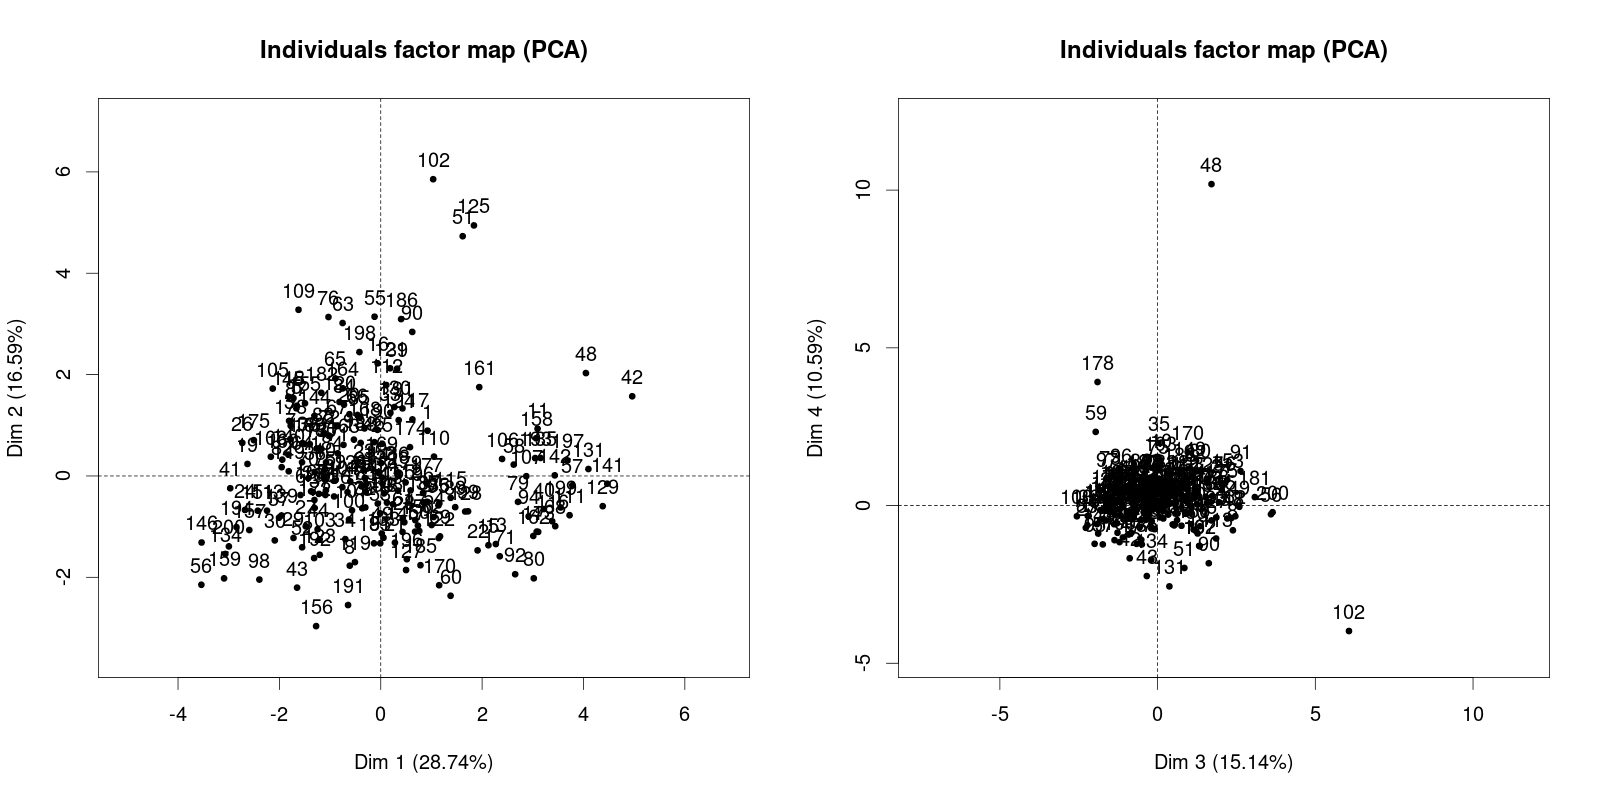
\includegraphics[width=\textwidth, keepaspectratio]{pcaind}
	\caption{Projection des individus sur les quatre premiers axes factoriels}
	\label{fig:pcaind}
\end{figure}
\FloatBarrier
\subsection{Analyse de la MCA}


\begin{figure}

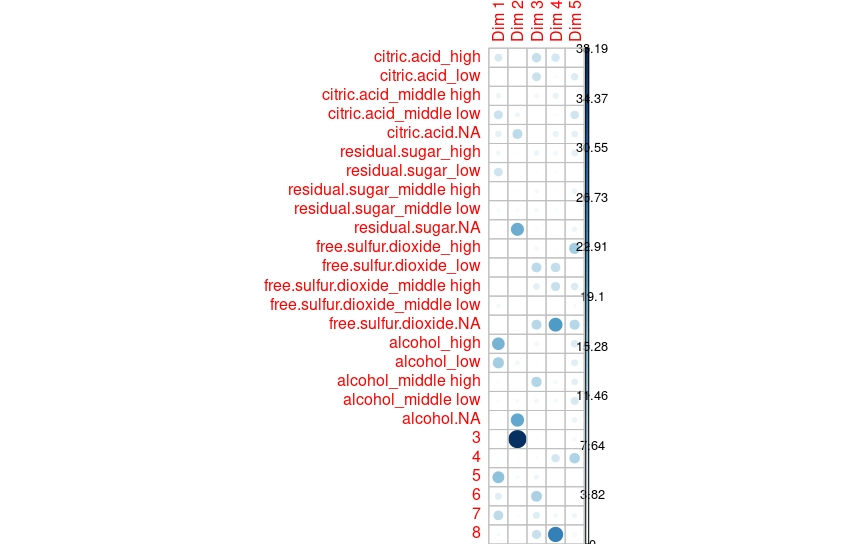
\includegraphics[width=\textwidth,keepaspectratio]{contrib}

\caption{Contributions des différente catégories}
\label{fig:contrib}
\end{figure}

\subsection{Clustering}

\begin{figure}[t]
\centering
\subfigure[single linkage]{
\includegraphics[width=.8\textwidth]{"single-pca"}
}
\subfigure[complete linkage]{
\includegraphics[width=.8\textwidth]{"complete-pca"}
}
\subfigure[ward]{
\includegraphics[width=.8\textwidth]{"ward-pca"}
}

\caption{Comparaison des méthode de clustering}
\label{fig:whatever}
\end{figure}




\section{Code R}
\lstset{language=R}
\begin{lstlisting}[breaklines]
##Code ici
\end{lstlisting}

\end{document}